% !TEX root = ../main.tex
% --+ 10.21 RG-E Target +-------------------------------------------------------
\begin{frame}{Run Group E (RG-E) Target}
    \label{10.21::rge_target}

    \begin{itemize}
        \item
            The RG-E target was designed to enhance our understanding of hadronisation in the nuclear medium.
            Its main observable is the \ef{hadronic multiplicity ratio}.

        \item
            To cancel time-dependent systematic effects, the system contains two targets of different density: a \ef{liquid deuterium} and a \ef{solid} target.

        \item
            The experiment is set to run at \ef{Hall B} of \ef{Jefferson Lab (JLab)}.
    \end{itemize}

    \begin{center}
        \begin{figure}[t]
            \centering{
                \fbox{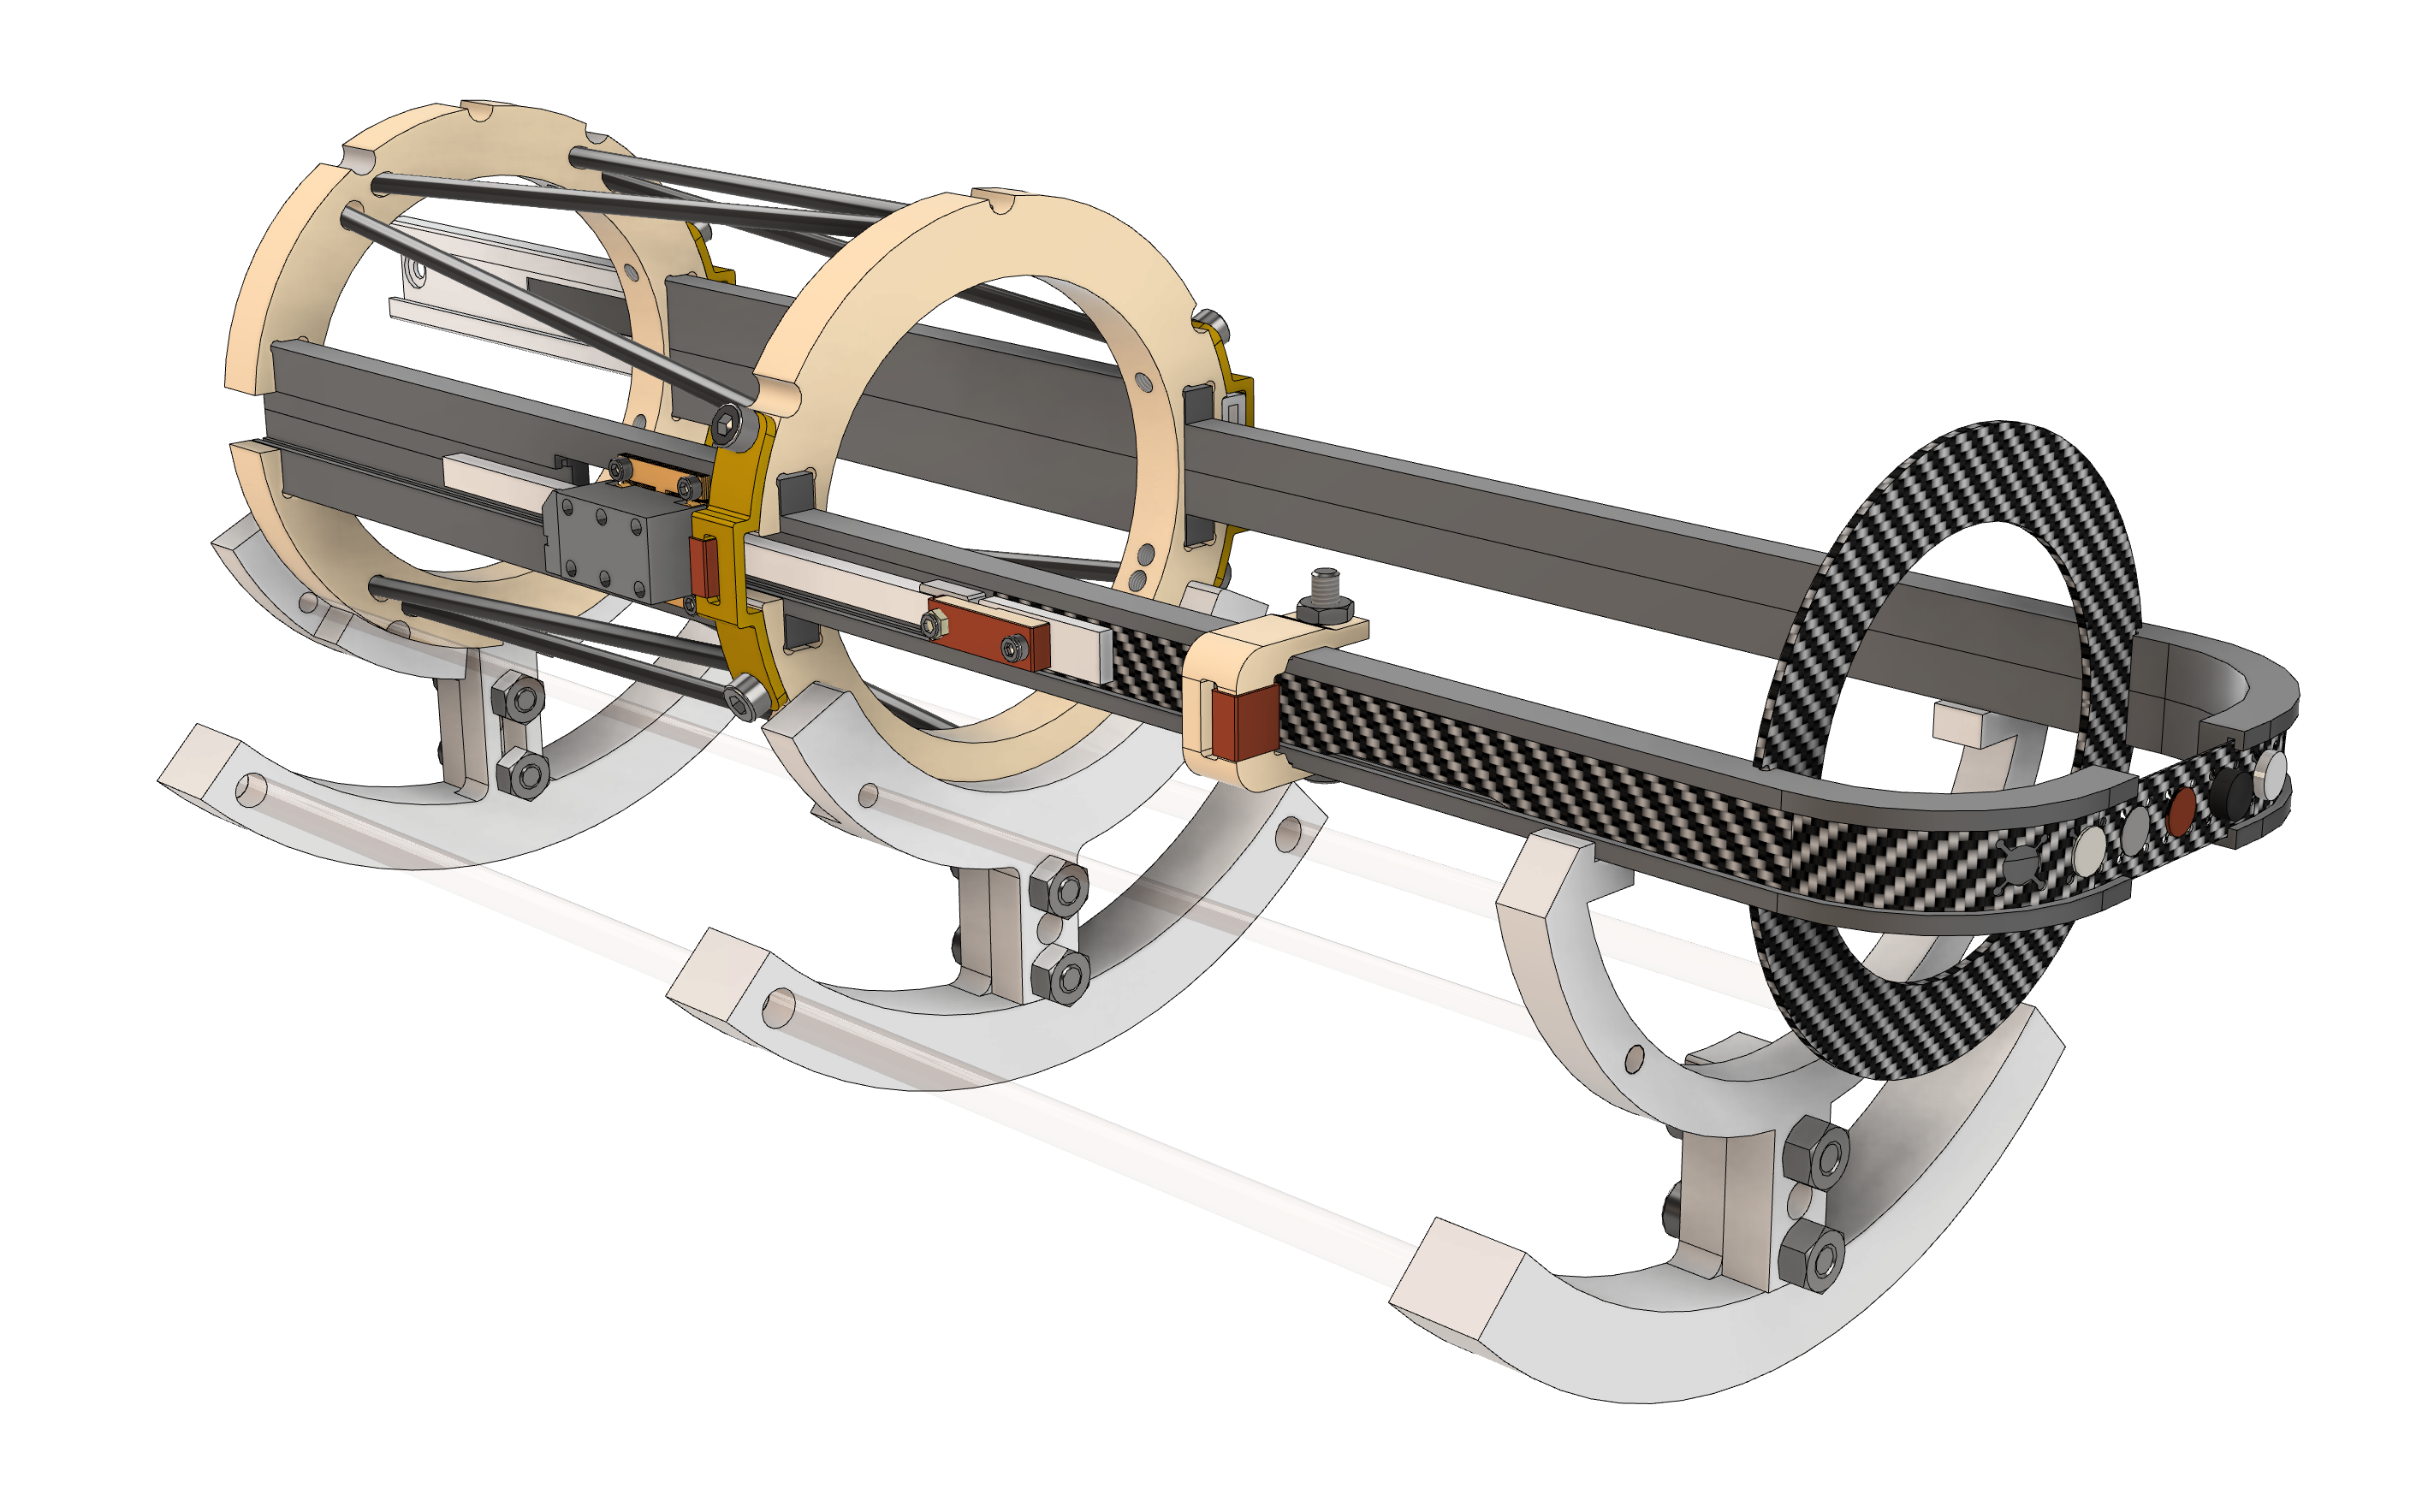
\includegraphics[width=0.5\textwidth]{21double_target.png}}
            }

            \scriptsize{\textit{
                RG-E target CAD render.
            }}
        \end{figure}
    \end{center}
\end{frame}
